\documentclass[a4paper,11pt]{article}
\usepackage{fullpage}
\usepackage[latin1]{inputenc}
\usepackage[T1]{fontenc}
\usepackage[normalem]{ulem}
\usepackage[english]{babel}
\usepackage{listings,babel}
\usepackage{palatino}
\lstset{breaklines=true,basicstyle=\ttfamily}
\usepackage{graphicx}
\usepackage{moreverb}
\usepackage{url}
\usepackage{tweaklist}
\renewcommand{\itemhook}{\setlength{\topsep}{0pt}\setlength{\itemsep}{0pt}}
\renewcommand{\enumhook}{\setlength{\topsep}{0pt}\setlength{\itemsep}{0pt}}

\title{TDC core test report}
\author{S\'ebastien Bourdeauducq}
\date{November 2011}
\begin{document}
\setlength{\parindent}{0pt}
\setlength{\parskip}{5pt}
\maketitle{}
\section{TODO}

\begin{figure}[h]
\centering
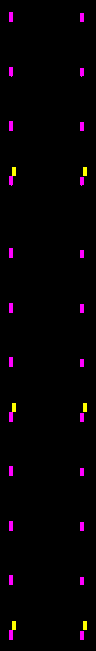
\includegraphics[width=1.6cm]{floorplan.png}
\caption{Floorplan of the delay lines and ring oscillators in FPGA Editor.}
\label{fig:floorplan}
\end{figure}

\begin{figure}[h]
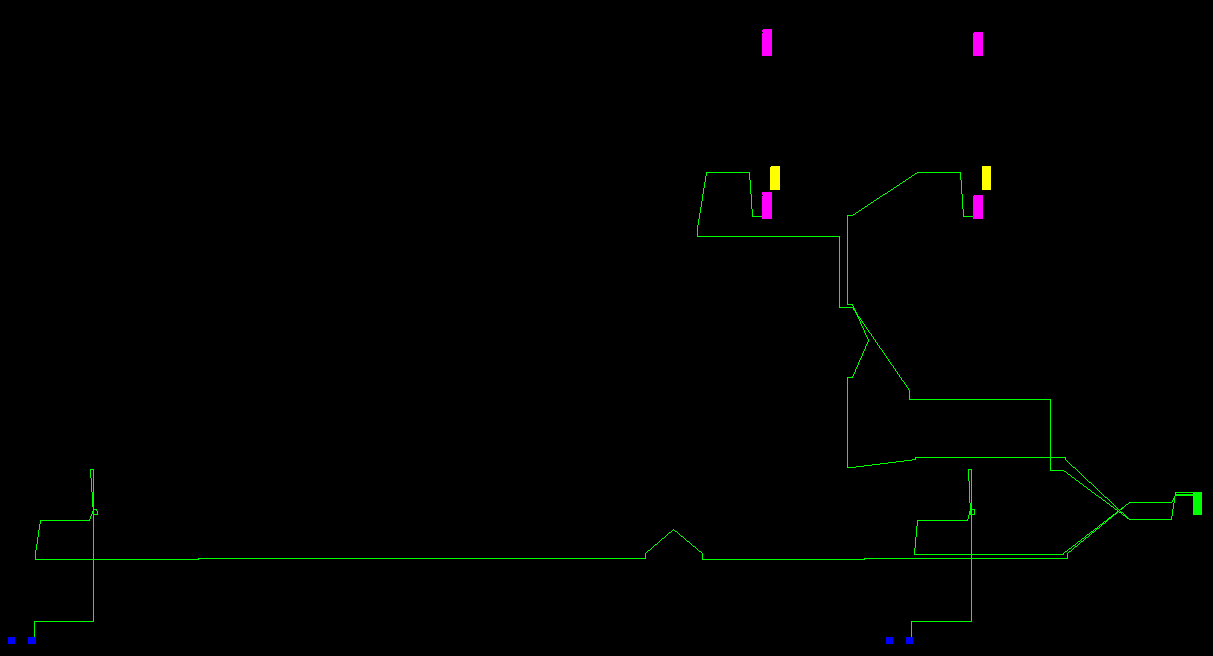
\includegraphics[width=\textwidth]{input_routes.png}
\caption{Input signal path in FPGA Editor.}
\label{fig:floorplan}
\end{figure}

\input{rofreq1_pdf.tex}

\input{rofreq2_pdf.tex}

\end{document}
